\subsection{Rich Calibration}
\textcolor{red}{This should include, description of the method (detector description
should be included in previous section), data selected, time required 
for this task, performance (before/after calibration) and stability of the constants
or variation as function of temperature/pressure. 
The overall performance, maybe also stability of the overall performance (PID 
or/and cherenkov angle resolution) could be together for calibration and alignment.}

The RICH automatic calibration consists of calibrating the RICH refractive index
and the Hybrid Photon Detectors (HPDs) images. Both these calibrations are
evaluated and updated every run.

The refractive index of the gas radiators depends on the ambient temperature and
pressure, and the exact composition of the gas mixture and so can change in
time.  These quantities are monitored to compute an expected refractive index,
but this does not have a high enough precision and needs to be corrected.  The
distribution of the difference between the reconstructed and expected Cherenkov
angle is fitted to extract the scale factor to correct the expected refractive
index.

\begin{figure}[h]
  \centering
  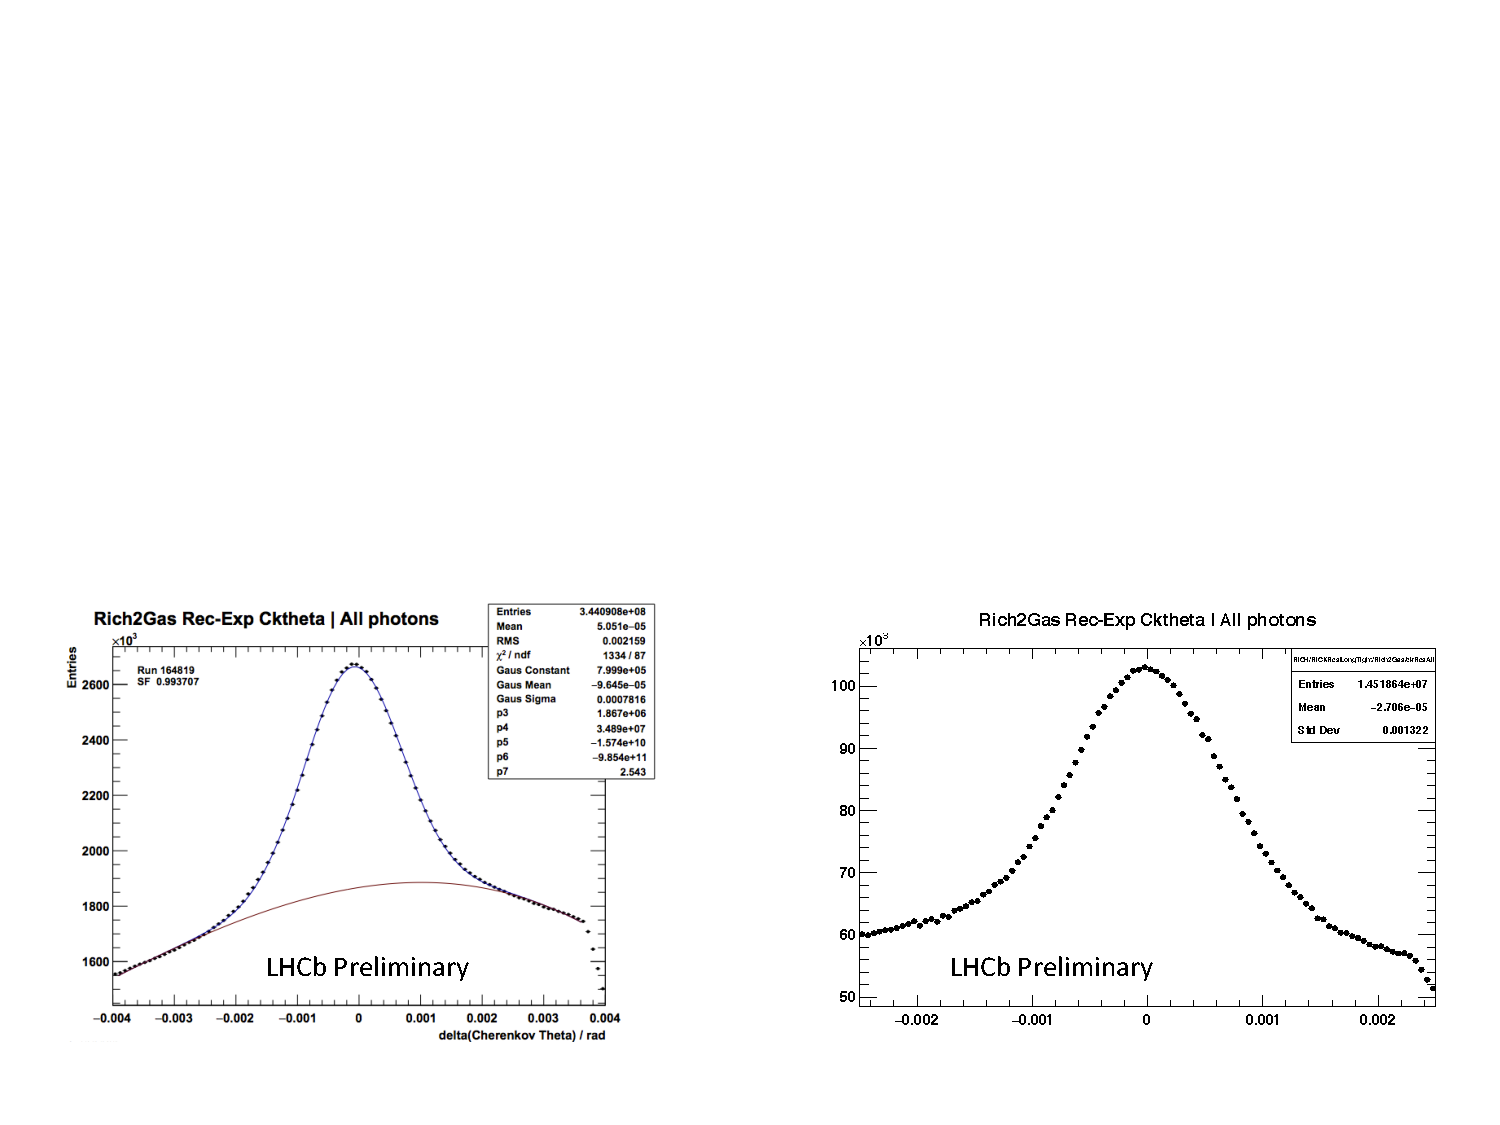
\includegraphics[width=8cm]{../figures/RichCalibration}
\caption{RICH cherenkov angle before (left) and after (right) the calibration,Caption to be written, 1st draft for the plot}
  \label{fig:RichCal}
\end{figure}

%due righe per spiegare HPD
HPDs are used to detect Cherenkov photons. They consist of vacuum tubes
separated from the radiator gas by a quartz window and a photocathode. The
photoelectrons produced are focused onto a silicon pixel array using an
accelerating voltage \cite{LHCb-DP-2012-003}.  The anode images are affected by
magnetic and electric fields, and so are cleaned and a Sobel filter \cite{Sobel}
is used to detect the edges. Figure \ref{fig:RichCal} shows the anode images
before and after this process. The evaluation of the new calibration constants
does not require an iterative procedure and can be obtained by fitting the
relevant distribution on a single node.

\begin{figure}[h]
  \centering
  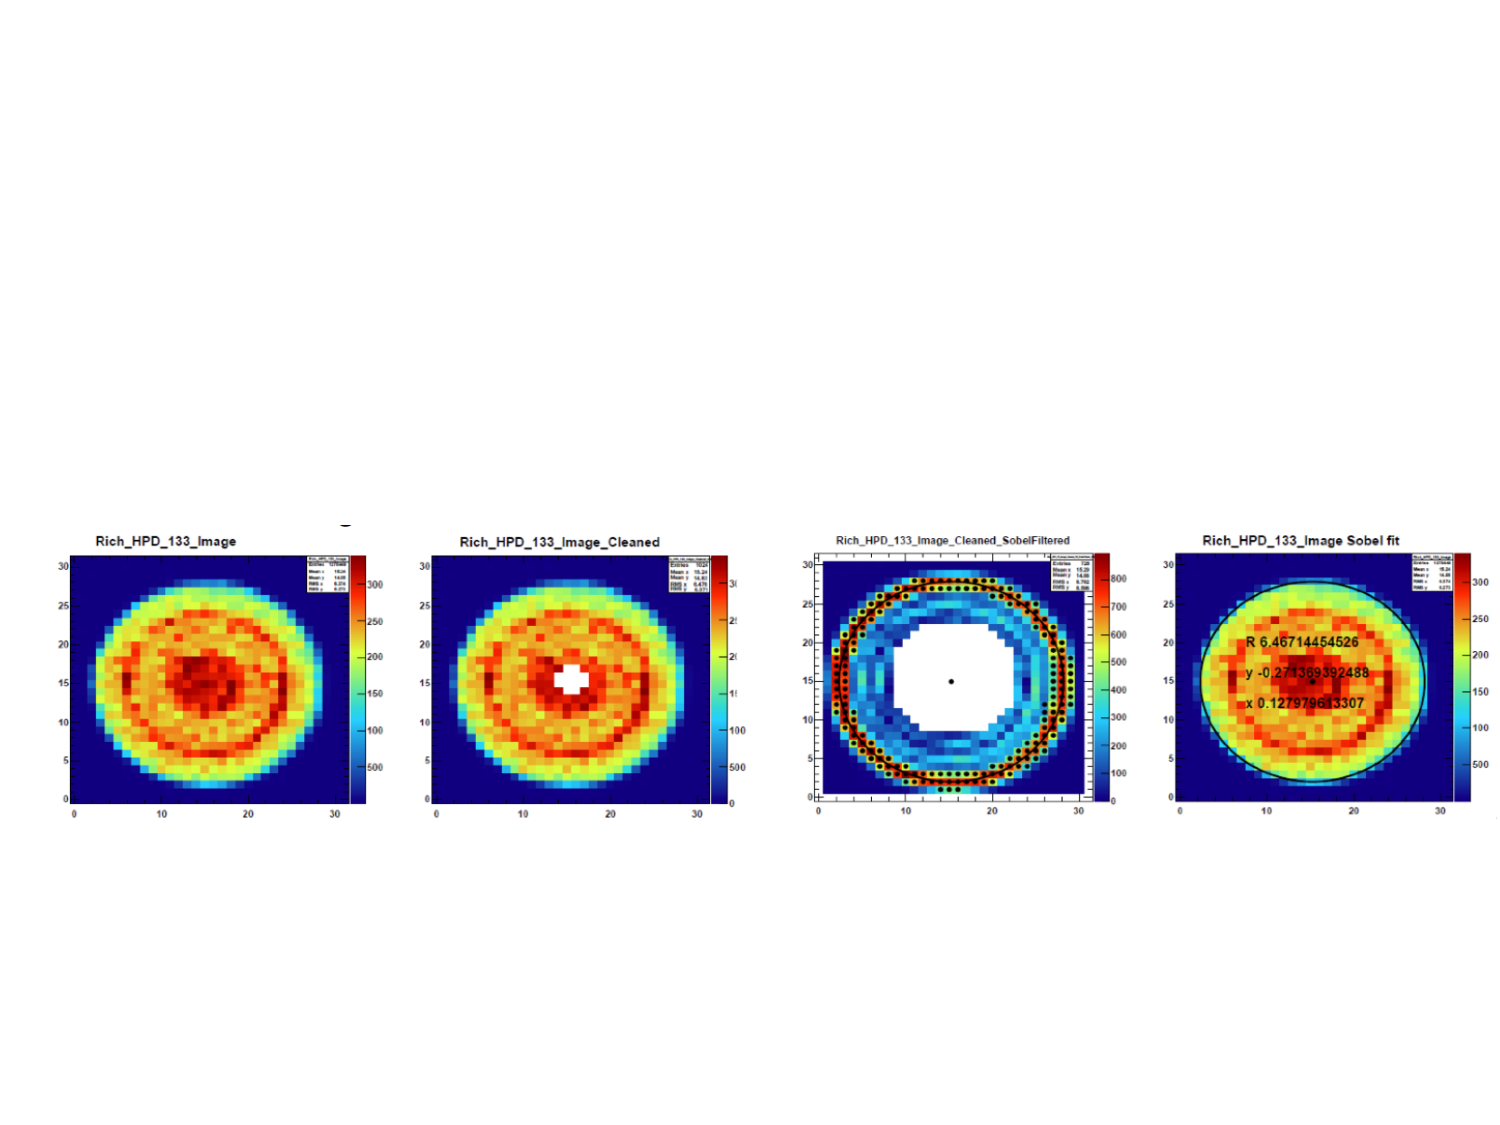
\includegraphics[width=8cm]{../figures/RichHPDCalibration}
\caption{RICH HPD anode images,Caption to be written, 1st draft for the plot.
%before (left) and after(right) the cleaning and applying the Sobel filter.
}
  \label{fig:RichHPDCal}
\end{figure}

